
%(BEGIN_QUESTION)
% Copyright 2006, Tony R. Kuphaldt, released under the Creative Commons Attribution License (v 1.0)
% This means you may do almost anything with this work of mine, so long as you give me proper credit

Shown here is a diagram for an {\it electronic} force-balance pressure transmitter:

$$\includegraphics[width=15.5cm]{i00207x01.eps}$$

Explain the following things in reference to this transmitter:

\begin{itemize}
\item{} What is a {\it flexure}?
\item{} How is the opposing force generated?
\item{} What does a {\it Hall Effect} sensor do?
\item{} How is an imbalance of force detected?
\item{} How would you incorporate a zero adjustment into this transmitter?
\item{} How would you incorporate a span adjustment into this transmitter?
\end{itemize}

\underbar{file i00207}
%(END_QUESTION)





%(BEGIN_ANSWER)

\noindent
{\bf Partial answer:}

A {\it flexure} is a thin strip of springy material, usually spring steel, designed to act as a frictionless fulcrum and/or a pivoting link.  Unlike bearings, flexures are usually not able to handle a lot of angular motion.

\vskip 10pt

{\it Hall Effect} sensors are used to detect magnetic fields.  They generate a DC voltage proportional to the magnitude and polarity of an applied magnetic field and the magnitude and direction of a perpendicular DC current:

$$V_{Hall} = K {IB \over x}$$

$$\includegraphics[width=15.5cm]{i00207x02.eps}$$

\filbreak

The operation of the Hall Effect sensor may not be clear to all readers.  It is oriented such that the magnetic field is parallel to the Hall Voltage axis and not perpendicular to it, when the beam is exactly level.  When the beam tips up or down, however, the magnetic flux lines passing from the ``North'' tip of the beam's magnet to the ``South'' tip of the stationary magnet to the left of the Hall Effect sensor will angle, passing through the Hall Effect sensor with a definite direction, either up or down, depending on which way the beam tips:

$$\includegraphics[width=15.5cm]{i00207x03.eps}$$

$$\includegraphics[width=15.5cm]{i00207x05.eps}$$

$$\includegraphics[width=15.5cm]{i00207x04.eps}$$

Thus, any output voltage from the Hall Effect sensor indicates an out-of-balance condition between the diaphragm and force motor.

%(END_ANSWER)





%(BEGIN_NOTES)

The questions on zero and span adjustments are probably the most interesting.  Remind your students that zero adjustments always {\it add} or {\it subtract}, while span adjustments always {\it multiply} or {\it divide}.

%INDEX% Measurement, pressure: electronic force-balance transmitter

%(END_NOTES)


